% Gemini theme
% https://github.com/anishathalye/gemini
%
% We try to keep this Overleaf template in sync with the canonical source on
% GitHub, but it's recommended that you obtain the template directly from
% GitHub to ensure that you are using the latest version.

\documentclass[6pt, final, xcolor=table]{beamer}
% ====================
% Packages
% ====================

\usepackage[T1]{fontenc}
\usepackage{lmodern}
\usepackage[size=a0]{beamerposter}
\usetheme{gemini}
\usecolortheme{gemini}
\usepackage{graphicx}
\usepackage{booktabs}
\usepackage{tikz}
\usepackage{pgfplots}
\usepackage{url}

% ====================
% Lengths
% ====================

% If you have N columns, choose \sepwidth and \colwidth such that
% (N+1)*\sepwidth + N*\colwidth = \paperwidth
\newlength{\sepwidth}
\newlength{\colwidth}
\setlength{\sepwidth}{0.025\paperwidth}
\setlength{\colwidth}{0.3\paperwidth}

\newcommand{\separatorcolumn}{\begin{column}{\sepwidth}\end{column}}
% ====================
% Colours
% ====================
\definecolor{tableGray}{RGB}{234, 234, 242}

% ====================
% Title
% ====================

\title{Who has used Heroin? An Application of Machine Learning in Drug Use Prediction}
\subtitle{Classification of Used Vs Never-Used}

%\institute[shortinst]{Imperial College London}
\author{Isaac Lee | Imperial College London}

% ====================
% Body
% ====================

\begin{document}
%\addtobeamertemplate{headline}{} 
%{\begin{tikzpicture}[remember picture, overlay]
%     \node [anchor=north east, inner sep=1.4cm]  at (current page.north east)
%    {\includegraphics[height=6cm]{green_imperial.png}};
%  \end{tikzpicture}}
 
\addtobeamertemplate{headline}{} 
{\begin{tikzpicture}[remember picture, overlay]
     \node [anchor=north west, inner sep=1.5cm]  at (current page.north west)
     {
\includegraphics[height=5cm]{white_text_border_imperial.png}};
  \end{tikzpicture}}
  
\begin{frame}[t]
\begin{columns}[t]
\separatorcolumn

\begin{column}{\colwidth}

  \begin{alertblock}{Introduction}

   In this project we look to answer the question: is it possible to distinguish
   between people who have used Heroin Vs people who have never used? We also look 
   to answer whether it is possible to build a model which predicts whether a given subject has taken
   Heroin at some point in their life.
  \end{alertblock}

  \begin{block}{The Data}

 This data set contains information for 1885 
 subjects on previous drug use for a vast array of drugs. (Note that in this project we will only be focusing on Heroin use). This data set comes from the UCI Machine Learning Repository$^{[1]}$
 In terms of the method, "an online survery methodology was employed to collect data" $^{[2]}$.
 For each person we have 12 features, which include a mix of categorical
 information and personality test score results.
 The Heroin column is the target vector, with binary values:
 \begin{itemize}
     \item  \textbf{0} : Never used Heroin at any point in the past
     \item  \textbf{1} : Used Heroin at least once 
 \end{itemize}
In terms of the balance of data, we have 1605 non-users and 280 who have used.
 \begin{figure}[h!]
    \centering
     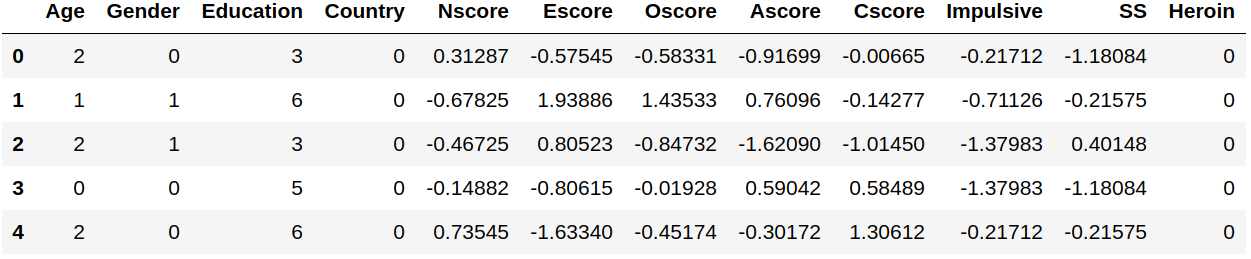
\includegraphics[scale=1.1]{df.png}
    \caption{The head of the data set.}
    \label{fig:dataset}
    \end{figure}
    
    \begin{itemize}
 \item \textbf{Age : } 0 : 18-24 | 1 : 25-34 | 2 : 35-44 | 3 : 45-54 | 4 : 55-64 | 5 : 65+
 \item \textbf{Gender : } 0 : Female | 1 : Male
 \item \textbf{Education : } 0 : Left school before 18 years 
 |  1 : Left school at 18 years \\
  2 : Some college or university but no certificate or degree \\
  3 : Professional certificate/diploma | 4 : University degree \\
  5 : Masters degree | 6 : Doctorate degree
 \item \textbf{Country : } 0 : UK \& Ireland | 1 : New Zealand \& Australia | 2 : USA \& Canada | 3 : Other \\
 \item \textbf{Personality Scores: } For the numerical features, we have information on "the Big Five" personality traits which
 are tested by the NEO-FFI-R: (N) Neuroticism | (E) Extraversion | (O) Openness to experience | (A) Agreeableness | (C) Conscientiousness $^{[3]}$
 \item \textbf{Impulsive \& SS: } Impulsive and (SS) Sensation Seeking which are measured by the Barrratt Impulsive Scale (BIS-11) $^{[3]}$
 \end{itemize}
 

  \end{block}

  \begin{block}{Feature Engineering/Encoding}
 \begin{itemize}
     \item \textbf{Encoding :} The original data set used nonlinear Categorical Principle Component Analysis for the nominal features and polychloric correlation for the ordinal features$^{[2]}$. I wanted to experiment with OneHot encoding, so instead I first converted to integer encoding and then used the pandas get\_dummies function to OneHot encode Gender and Country.  
  \item \textbf{Binarization :} The original data set contains four classes, such as: "used in the past day", "used in the past month" e.t.c. In order to simplify the problem
 we convert to: "never used" and "used at some point in the past".
  \item \textbf{Country Combinations :} Several countries have very few participants and so
  we combine geographically/culturally similar countries as seen above.
  \item \textbf{Education Combinations :} Originally there existed several classes of people who left school before 18. To simplify things we combine into the 0 : Left school before 18 years education class.
 \end{itemize}
\hrule
\vspace{2mm}

\begin{description}
    \small{\item [{[1]}] Evgeny M. Mirkes Elaine Fehrman, Vincent Egan.} \footnotesize{UCI machine learning repository, 2016} 
    \small{\item [{[2]}] E. Fehrman, A. K. Muhammad, E. M. Mirkes, V. Egan, and A. N. Gorban.} \\
    \footnotesize{The five factor model of personality and evaluation of drug consumption risk, 2017.}
    \small{\item [{[3]}] Michael C. Ashton.} \footnotesize{Chapter 2 - Personality Traits and the Inventories that Measure Them. \\
    Academic Press, San Diego, second edition edition, 2013.}
    
\end{description}




  \end{block}







\end{column}

\separatorcolumn

\begin{column}{\colwidth}

  \begin{block}{Feature Exploration}
    We now explore the distributions/correlations for each feature with count, KDE and correlation
    plots:
  \begin{figure}[h!]
    \centering
     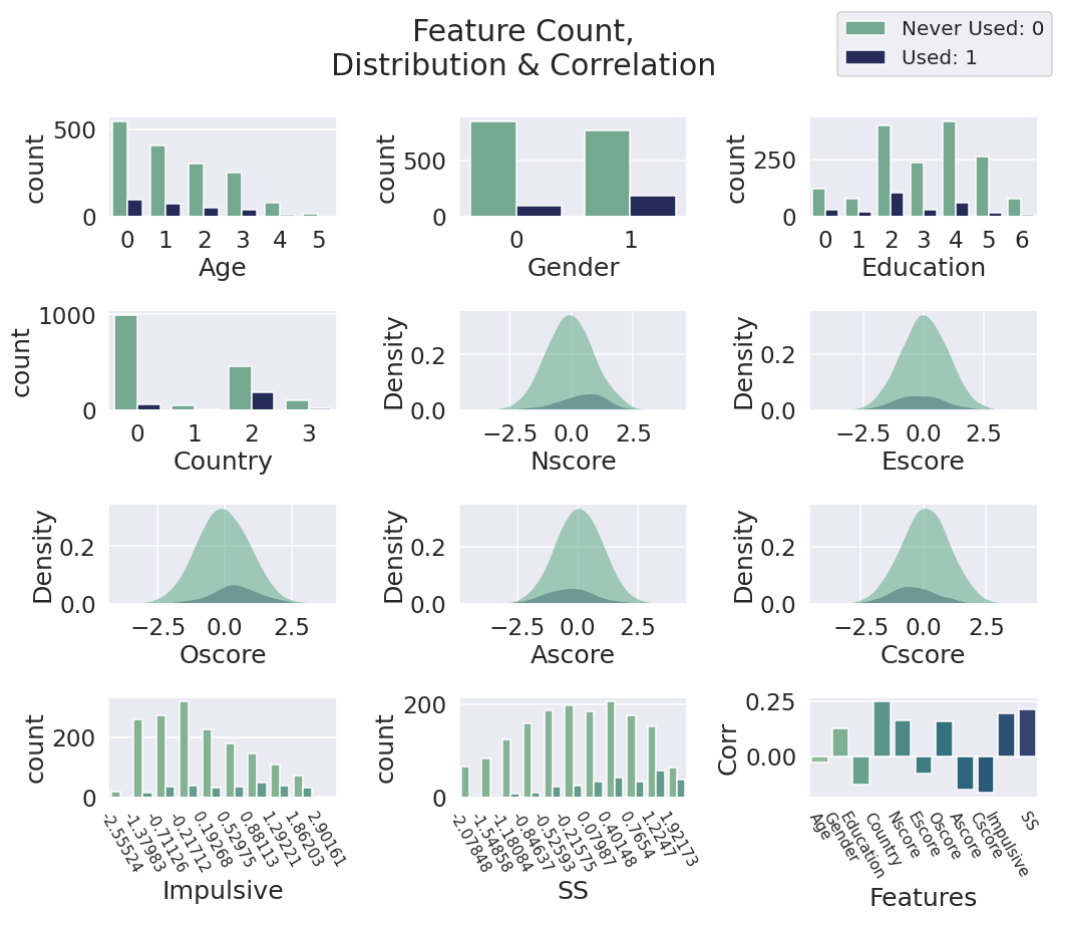
\includegraphics[scale=1.2]{feature_plots.png}
    \caption{Exploring the distribution and correlation of each feature.}
    \label{fig:feature_plots}
    \end{figure}
    \heading{Interpretations}
    Clearly from these plots it appears that Nscore, Escore, Oscore, Ascore and Cscore
    are normally distributed, however the other features are not, with non-central means.
    Also when considering the correlation of features with Heroin use, it appears that Country, SS and Impulsive are most correlated, suggesting that they will have greater importance in our models.

  \end{block}

\begin{block}{Model Creation}
\heading{Train Test Split}
We use Sklearn to split our data into stratified 80\% training and 20\% testing data.
 \heading{Naive Bayes}
Naive Bayes will provide a good baseline model for comparison due to it's simplicity. 
We use the Sklearn library to fit the Naive Bayes model to our training data.
Naive Bayes uses Bayesian Inference to get information on the posterior 
distribution. So for every vector of features we can calculate the probability of obtaining
either a 1 or a 0 given the data we have observed, and predict the most likely. Note that we assume independence of features, when clearly this is not the case $^{[4]}$.

 \heading{XGBoost}
    For a more complex model we turn to XGBoost.
    This algorithm uses an ensemble approach with many "weak learners" which are weighted according to their
    error $^{[4]}$. We use the xgboost python library to fit the model to our training data,
    and then we use Sklearn GridSearchCV to find the best possible parameters using
    cross validation.  

\end{block}

\hrule
\begin{description}
    \small{\item [{[4]}] Tibshirani R. Friedman J. H. Hastie, T.} \\
    \footnotesize{The elements of statistical learning: Data mining, inference, and prediction : with 200 full-color illustrations. New York : Springer, New York, second edition edition, 2001.} 
\end{description}

\end{column}

\separatorcolumn

\begin{column}{\colwidth}

\heading{Random Forest}
    Finally for our third model, we try Random Forest, which is another decision tree
    algorithm. The basic idea of Random Forest is to create a "Forest" of smaller decision trees made from random subsets of features, which separate samples based on their "Gini Impurity" and then using ensemble techniques the results are combined $^{[4]}$. As before we tune our parameters using GridSearchCV in several iterations.
  \begin{figure}[h!]
    \centering
     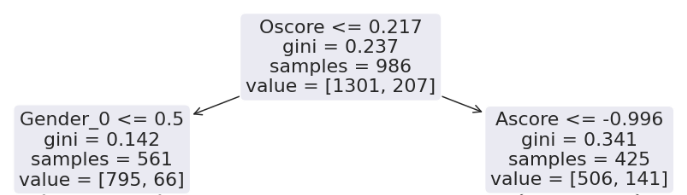
\includegraphics[scale=1.3]{smaller_rf_tree.png}
    \caption{An example of some nodes from a decision tree.}
    \label{fig:method}
    \end{figure}  


  \begin{block}{Model Results}

    In the table below we provide the results on both the training and testing data for each
    algorithm. Also we use 5-fold cross validation on the \textbf{whole} data set for another
    measure of accuracy. Finally we have the standard error for the 5-fold cross validation
    results for each model.

  \begin{figure}[h!]
    \centering
     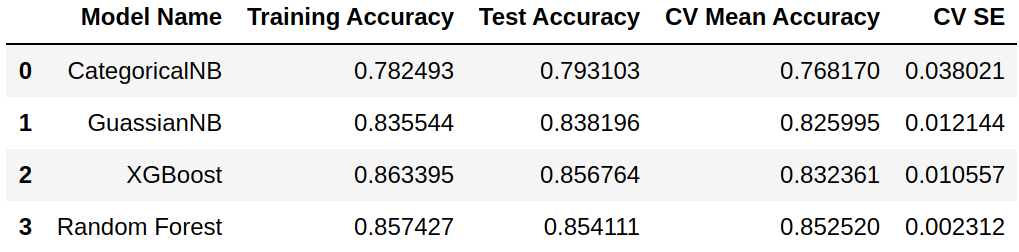
\includegraphics[scale=1.5]{model_results.png}
    \caption{Model Results.}
    \label{fig:method}
    \end{figure}  
    
\heading{Interpretation of Results}
Firstly we note that the accuracy for XGBoost and Random Forest is decently higher than
Naive Bayes, which is to be expected. Also note that we are getting some overfitting on our
XGBoost model, since the training data accuracy is higher than the test data accuracy.
Also whilst the accuracy for XGBoost on the test data is higher than Random Forest,
when we look at the 5-fold cross validation scores Random Forest is the clear winner,
with it also having a much lower standard error than any of the other models.
It is also interesting to consider the confusion matrix heatmaps for each model, because they show that the decision tree based algorithms actually performed worse when identifying users, tending to largely favour non-users.
 
  \begin{figure}[h!]
    \centering
     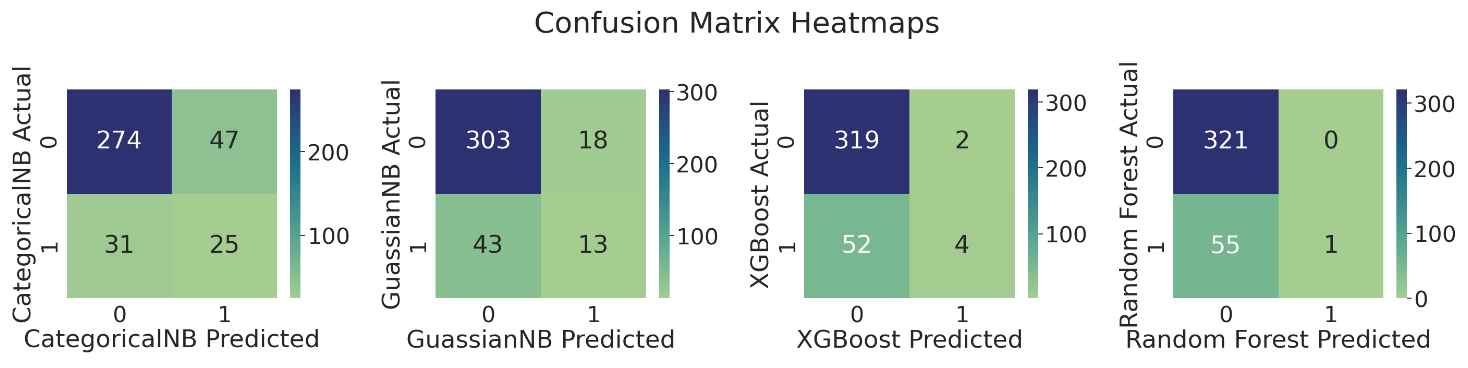
\includegraphics[scale=0.9]{conf_mat_heatmaps.png}
    \caption{Comparing predicted values with actual for each model.}
    \label{fig:conf_matrix}
    \end{figure}   

  \end{block}
  \begin{alertblock}{Conclusions}
We can now answer the questions we first set out:
Yes! (Accepting an error of approx 15\%), it is possible to predict whether or not
someone has used Heroin at some point in their life, suggesting
that (most) Heroin users have distinguishable characteristics.
  \end{alertblock}
  
  \begin{block}{GitHub \& Oral Presentation}
  \begin{itemize}
      \item GitHub Repository for source Jupyter Notebook code:  \small{\url{https://github.com/isaacjeffersonlee/Project_6_Y1_ICL}}
      \item Oral Presentation Link:  \\
      \small{\url{https://imperial.cloud.panopto.eu/Panopto/Pages/Viewer.aspx?id=0084d56a-fe27-4892-9744-ad4500c942b9}}
  \end{itemize}

% \footnotesize{\bibliographystyle{unsrt}\bibliography{poster}}
 

  \end{block}

\end{column}

\separatorcolumn
\end{columns}
\end{frame}

\end{document}
